\documentclass[12pt,a4paper]{article}
\usepackage{ctex}
\usepackage{amsmath,amscd,amsbsy,amssymb,latexsym,url,bm,amsthm}
\usepackage{epsfig,graphicx,subfigure}
\usepackage{enumitem,balance}
\usepackage{wrapfig}
\usepackage{mathrsfs, euscript}
\usepackage[usenames]{xcolor}
\usepackage{hyperref}
\usepackage[vlined,ruled,commentsnumbered,linesnumbered]{algorithm2e}
\usepackage{float}
\usepackage{array}
\usepackage{diagbox}
\usepackage{color}
\usepackage{indentfirst}
\usepackage{fancyhdr}
\usepackage{gensymb}
\usepackage{geometry}
\usepackage{setspace}
\usepackage{aurical}
\usepackage{times}
\usepackage{caption}
\usepackage{fontspec}
\usepackage{booktabs}
\usepackage{listings}
\usepackage{xcolor}
\setmainfont{Times New Roman}

\newtheorem{theorem}{Theorem}[section]
\newtheorem{lemma}[theorem]{Lemma}
\newtheorem{proposition}[theorem]{Proposition}
\newtheorem{corollary}[theorem]{Corollary}
\newtheorem{exercise}{Exercise}[section]
\newtheorem*{solution}{Solution}
\theoremstyle{definition}

\newcommand{\postscript}[2]
 {\setlength{\epsfxsize}{#2\hsize}
  \centerline{\epsfbox{#1}}}

\renewcommand{\baselinestretch}{1.05}

\setlength{\oddsidemargin}{-0.365in}
\setlength{\evensidemargin}{-0.365in}
\setlength{\topmargin}{-0.3in}
\setlength{\headheight}{0in}
\setlength{\headsep}{0in}
\setlength{\textheight}{10.1in}
\setlength{\textwidth}{7in}
\makeatletter \renewenvironment{proof}[1][Proof] {\par\pushQED{\qed}\normalfont\topsep6\p@\@plus6\p@\relax\trivlist\item[\hskip\labelsep\bfseries#1\@addpunct{.}]\ignorespaces}{\popQED\endtrivlist\@endpefalse} \makeatother
\makeatletter
\renewenvironment{solution}[1][Solution] {\par\pushQED{\qed}\normalfont\topsep6\p@\@plus6\p@\relax\trivlist\item[\hskip\labelsep\bfseries#1\@addpunct{.}]\ignorespaces}{\popQED\endtrivlist\@endpefalse} \makeatother

\begin{document}
\noindent
%==========================================================
\noindent\framebox[\linewidth]{\shortstack[c]{
\Large{\emph{模型评价与模型改善}}\vspace{1mm}\\
CS245 \quad 数据科学基础 \quad 陆朝俊 \vspace{1mm} \\
叶泽林 515030910468}}

\section{问题描述}



\section{解决方案\protect\footnote{本次作业的所有代码实现可参见附录 \ref{apd:code}}}

\subsection{数据集的建立及模型的选择}


\subsection{探索模型单独工作的性能}

\begin{enumerate}
\item \textbf{直接划分训练集和测试集}

无可奉告

\item \textbf{交叉验证}

\item \textbf{网格搜索}
\end{enumerate}

\subsection{探索模型组合工作的性能}

\section{结果展示}

\subsection{模型单独工作的性能}
\label{sec:pca_res_com}

\subsubsection{直接划分训练集和测试集}

\subsubsection{交叉验证}

\subsubsection{网格搜索}

\subsection{模型组合工作的性能}

\subsubsection{bagging}

\subsubsection{boosting}


\newpage
\begin{appendix}
	\section{附录}
	\subsection{Boston数据集特征信息}
	\label{apd:boston_char}
	\begin{table}[H]
		\renewcommand\arraystretch{1.35}
		\caption{Boston数据集特征信息}
		\label{tab:boston_char}
		\centering
		
		\begin{tabular}{c|c|c}
			\centering
			编号 & 特征名 & 特征含义 \\
			\hline
			1 & CRIM & 城镇人均犯罪率 \\
			2 & ZN & 住宅用地超过 25000 sq.ft. 的比例 \\
			3 & INDUS & 城镇非零售商用土地的比例 \\
			4 & CHAS & 查理斯河空变量(如果边界是河流,则为1;否则为0) \\
			5 & NOX & 一氧化氮浓度 \\
			6 & RM & 住宅平均房间数 \\
			7 & AGE & 1940 年之前建成的自用房屋比例 \\
			8 & DIS & 到波士顿五个中心区域的加权距离 \\
			9 & RAD & 辐射性公路的接近指数 \\
			10 & TAX & 每 10000 美元的全值财产税率 \\
			11 & PTRATIO & 城镇师生比例 \\
			12 & B & 1000(Bk-0.63)\^ 2,其中 Bk 指代城镇中黑人的比例 \\
			13 & LSTAT & 人口中地位低下者的比例 \\			
		\end{tabular}
	\end{table}
	
	\subsection{PCA算法在主成分个数为3时的进一步可视化}
	\label{apd:vis3}
	
	\begin{figure}[H]
		\centering
		\subfigure{
		    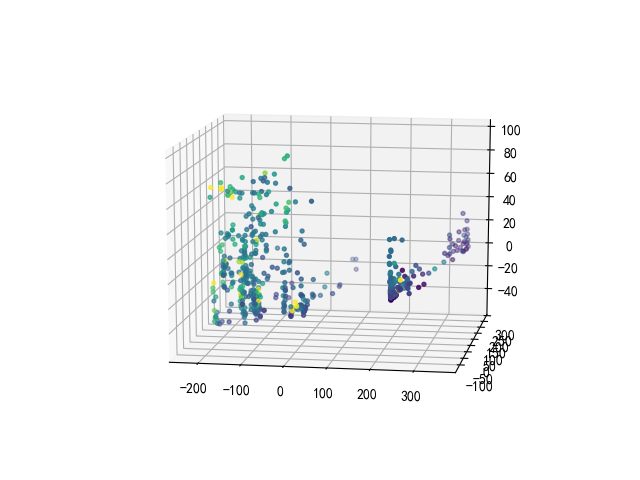
\includegraphics[width=0.3\linewidth]{img/pca-3-0.png}
		}
		\subfigure{
			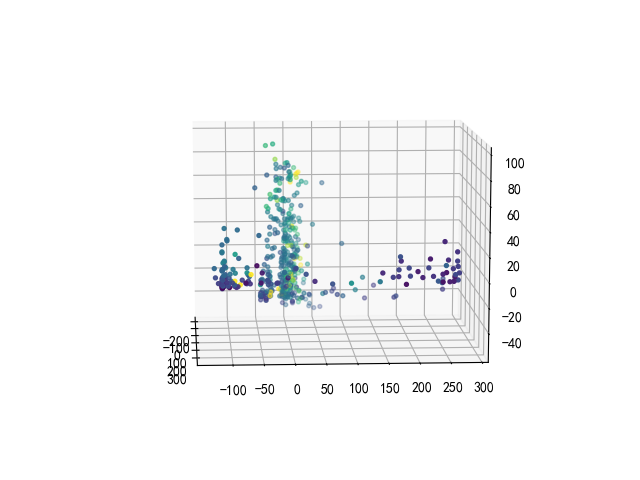
\includegraphics[width=0.3\linewidth]{img/pca-3-1.png}
		}
		\subfigure{
			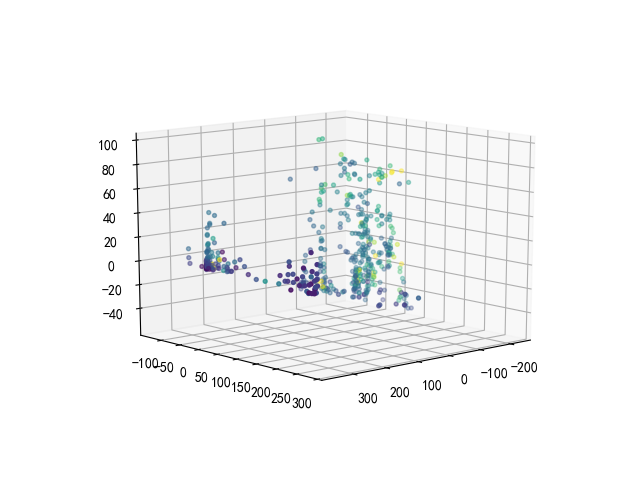
\includegraphics[width=0.3\linewidth]{img/pca-3-2.png}
		}
		\subfigure{
		    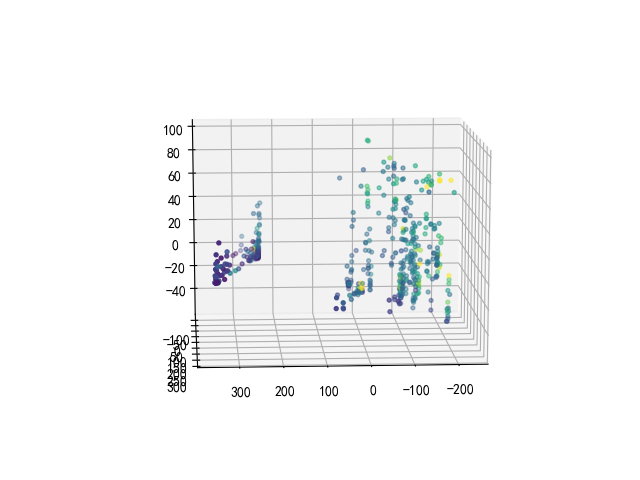
\includegraphics[width=0.3\linewidth]{img/pca-3-3.png}
		}
		\subfigure{
			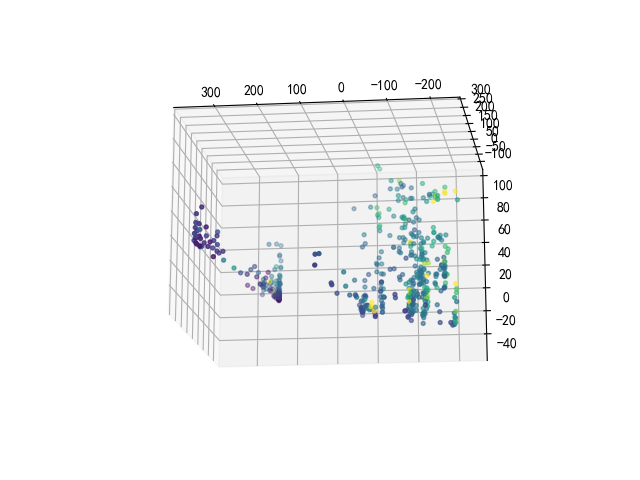
\includegraphics[width=0.3\linewidth]{img/pca-3-4.png}
		}
		\subfigure{
			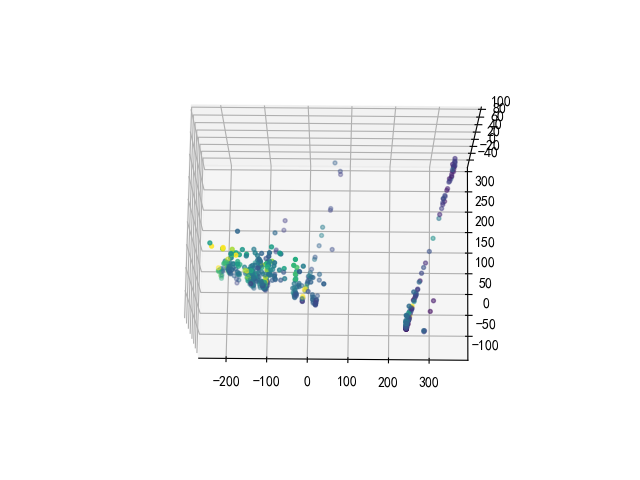
\includegraphics[width=0.3\linewidth]{img/pca-3-5.png}
		}
		\caption{PCA效果进一步可视化(主成分个数为3时)}
		\label{fig::pca_vis3}
	\end{figure}
	
	\subsection{主要代码}
	\label{apd:code}
	
	\begin{lstlisting}[language=Python,
	numbers=left,
	keywordstyle=\color{blue!70},
	frame=shadowbox,
	breaklines=True]
import matplotlib.pyplot as plt
plt.rcParams['font.sans-serif'] = ['SimHei']    # display Chinese
plt.rcParams['axes.unicode_minus'] = False      # display minus sign
from mpl_toolkits.mplot3d import Axes3D
from sklearn import datasets
from sklearn.decomposition import PCA

import os
import time

class bostonAnalyzer(object):
    def __init__(self):
        # load dataset
        self.dataset = datasets.load_boston()
        self.data = self.dataset.data
        self.target = self.dataset.target
        
        # for plot
        self.var = []
        self.t = []

        if not os.path.exists('report/img'):
            os.makedirs('report/img')

    def run(self, vis=False):
        '''
        Run PCA for 1-13 dimensions
        :param vis: True: plot dim 1-3; False: not plot
        '''

        self.var.clear()
        self.t.clear()

        with open('report/result.txt', 'w') as f:
            for i in range(13):
                t = time.time()
                pca_op = PCA(n_components=i)
                pca_res = pca_op.fit_transform(self.data)
                t = time.time() - t

                self.var.append(pca_op.explained_variance_ratio_.sum())
                self.t.append(t)

                # write log
                f.write('###### Dimension %d ######\n' % i)
                f.write(str(pca_res.shape) + '\n')
                f.write(str(pca_op.explained_variance_ratio_) + '\n')
                f.write(str(pca_op.explained_variance_ratio_.sum()) + '\n')
                f.write(str(t) + '\n\n')

                # visualize for debug & plot
                if vis:
                    if i == 1:
                        # plot 1 dimension
                        plt.scatter(pca_res[:, 0], pca_res[:, 0], s=14, c=self.target)
                        plt.savefig('report/img/pca-%d' % i)
                        plt.show()
                    elif i == 2:
                        # plot 2 dimensions
                        plt.scatter(pca_res[:,0], pca_res[:,1], s=8, c=self.target)
                        plt.savefig('report/img/pca-%d' % i)
                        plt.show()
                    elif i == 3:
                        # plot 3 dimensions
                        ax = plt.subplot(projection='3d')
                        ax.scatter(pca_res[:, 0], pca_res[:, 1], pca_res[:, 2], s=8, c=self.target)
                        plt.savefig('report/img/pca-%d' % i)
                        plt.show()

    def show(self):
        '''
        Show the basic info of Boston dataset & plot k-lines
        '''
        print(self.data.shape)
        print(self.target.shape)
        self._k_line_radio()
        self._k_line_time()

    def _k_line_radio(self):
        '''
        Plot k-line of variant radio
        '''
        x = list(range(len(self.var)))
        plt.scatter(x, self.var, s=14, c='r')
        plt.plot(x, self.var)
        plt.xlabel('主成分个数')
        plt.ylabel('降维后各特征方差比例之和')
        plt.savefig('report/img/kline-radio')
        plt.show()

    def _k_line_time(self):
        '''
        Plot k-line of time
        '''
        x = list(range(len(self.t)))
        plt.scatter(x, self.t, s=14, c='r')
        plt.plot(x, self.t)
        plt.xlabel('主成分个数')
        plt.ylabel('PCA算法消耗时间(s)')
        plt.savefig('report/img/kline-time')
        plt.show()

if __name__ == '__main__':
    bA = bostonAnalyzer()
    bA.run(True)
    bA.show()
	\end{lstlisting}
	
\end{appendix}

%========================================================================
\end{document}